\documentclass[a4paper,11pt]{article}
\usepackage[utf8]{inputenc}
\usepackage{amsmath}
\usepackage{amsfonts}
\usepackage{amssymb}
\usepackage{graphicx}
\usepackage{braket}

\numberwithin{equation}{section}
\renewcommand\thesubsection{\alph{subsection}}
\newcommand{\bvp}[1]{\mathbf{#1}'}
\newcommand{\bv}[1]{\mathbf{#1}}

\newcommand{\aval}{e^{-i\hbar\frac{15}{4}t}}
\newcommand{\bval}{e^{-i\hbar\frac{3}{4}t}}
\newcommand{\cvalp}{e^{i\hbar 3t}}
\newcommand{\cvaln}{e^{-i\hbar 3t}}

%opening
\title{Quantum II HW5}
\author{Vincent Baker}

\begin{document}

\maketitle

\section{Problem 1}
We find the first 5 Fourier coefficients of $ \frac{1}{3+2\cos{\theta}}$ using numerical integration of $\frac{1}{2\pi}\int_{-\pi}^{\pi}\frac{e^{-ik\theta}}{3+2\cos{\theta}} d\theta $.
\begin{gather}
 k_0 = \frac{2.8099}{2\pi}\\
 k_1 = \frac{0.2685}{2\pi}\\
 k_2 = \frac{0.1579}{2\pi}\\
 k_3 = \frac{0.0486}{2\pi}\\
 k_4 = \frac{-0.0323}{2\pi}
\end{gather}

\section{Problem 2}
The problem is set up in p2.m. The results are shown below.\\
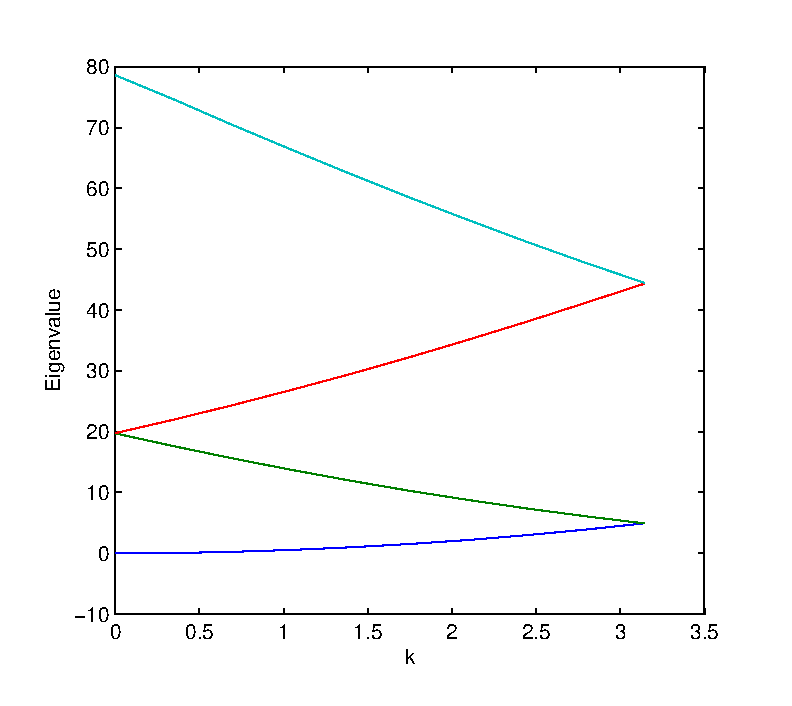
\includegraphics{p2}
\\

\section{Problem 3}
The problem is set up in p3.m. The results are shown below.
100 steps are taken along each segment.\\
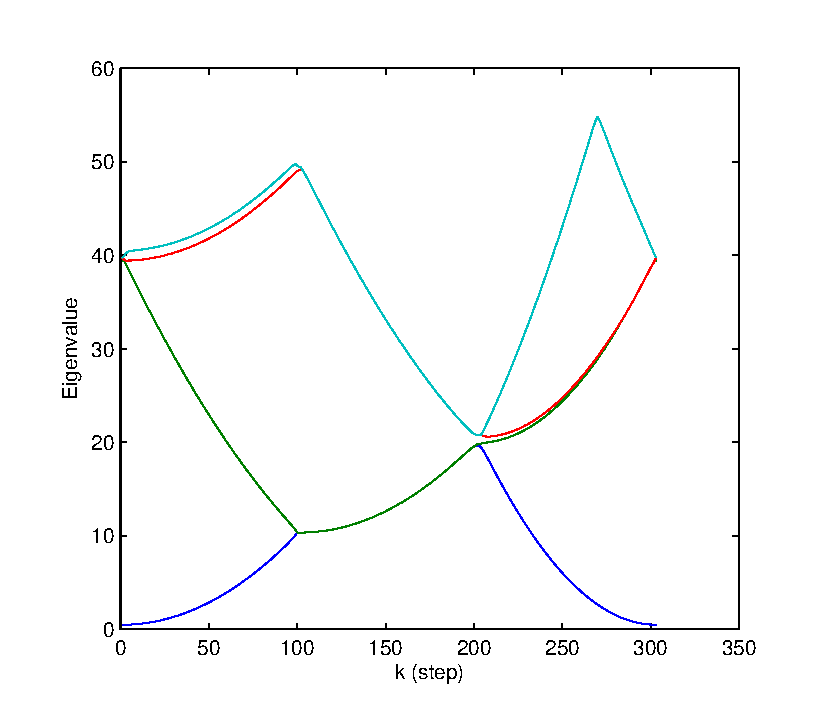
\includegraphics{p3}


\end{document}
